% !TEX TS-program = xelatex+makeindex+bibtex
% !TEX encoding = UTF-8
% !TEX root = ../chalice2sil_report_klauserc.tex

\section{Evaluation}\label{sct:eval}

\subsection{SIL as a translation target/verification intermediate language}
One of the primary goals of writing Chalice2SIL was to gather experience working with SIL, both as a translation target and as a verification intermediate language. 

\subsubsection{Encoding of loops}
At the time we started this project, SIL did not have a dedicated \lstinline[language=Chalice]!while! loop node. 
Instead, programs were to be encoded as a flat directed graph of basic blocks: a control-flow graph (CFG).
Loops were encoded as cycles with the ``backwards'' pointing edge explicitly marked (so that tools could traverse the CFG as an acyclic graph by ignoring those back edges).
Unfortunately, Silicon -- our verifier for SIL -- can currently only handle \lstinline[language=Chalice]!while! loops as they appear in Chalice. 
In those early days, Silicon would pattern match against the CFG to find \lstinline[language=Chalice]!while! loops and extract their components (condition, invariant, body), essentially lifting the program back up to the abstraction level of Chalice in terms of control flow.
If Chalice, which only supports \lstinline[language=Chalice]!while! loops, were the only source language that SIL ever had to support, this approach would have been fine.
But since the idea behind SIL was to eventually have multiple front ends, we decided to capture the fact that we currently can only verify \lstinline[language=Chalice]!while! loops -- and not arbitrary control flow graphs -- in the language.
As a result a explicit loop node was added to the SIL control-flow graph.

\subsubsection{Syntactic distinction between assertions and program expressions}
Currently, SIL distinguishes between assertions (logical formulae and accessibility predicates) and program expressions on a syntactic level. 
Some language elements require assertions as operands (e.g., \lstinline[language=SIL]!exhale!) while others only accept program expressions (e.g., method arguments).
In the current implementation of the SIL abstract syntax tree (AST), there are two distinct and unrelated types: the type of assertions and the type of program expressions.
Having the Scala compiler enforce that we never construct a SIL program where an accessibility predicate is used as a method argument is nice in theory, but proved to be more cumbersome than necessary in practice.

\begin{description}
\item[Only a partial solution] It is still possible to write translators that try to create illegal assertions and will fail due to runtime\footnote{In the context of $X$-to-SIL-translators, ``runtime'' refers to the execution of the translator.} checks built into the SIL AST.
While it would seem better to check as many properties statically as possible, only ending up with partial checks can result in a false sense of security. 
The SIL AST API is not exception-free and translators should be prepared deal with exceptions.
\item[Code duplication] Logical formulae and program expressions have a lot in common, e.g. logical operators or literal values. 
Distinguishing between a program-level \lstinline[language=Chalice]!true! and and an assertion-level \lstinline[language=Chalice]!true! has little benefit and at the same means that both producers and consumers of SIL need to have two pieces of code that handle boolean literals.
Since the Scala types of assertions and program expressions are unrelated, there is absolutely no opportunity for code reuse.
\item[Translation from Chalice] The Chalice compiler does not distinguish between assertions and program expressions on a syntactic level and instead enforces restrictions on where certain expressions can appear in semantic checks during type checking. 
Unfortunately, this makes syntax driven translation from Chalice to SIL highly ambiguous. 
The translator will come across many Chalice expressions where it is not a priori clear whether to translate them as SIL assertions or as SIL program expressions. 
For instance \ch{5 == 3} can be translated using the equality assertion \sil{\text{\lstinline[language=SIL]!5 == 3!}} or by first applying the integer equality domain function \lstinline!intEQ! and then lifting the resulting boolean program value up to assertion-level using the boolean domain predicate \lstinline!eval!: \sil{\text{\lstinline[language=SIL]!eval(intEQ(5,3))!}}.

Not all expressions can be translated either way and to find out which translation scheme is the correct one often requires having a look at the entire expression tree and not just the outermost expression node. 
This can mean that a translator needs to walk through Chalice expressions twice, either just trying both translation schemes in turn or first analysing the expression and then deciding on a translation scheme to use.

\item[Need to convert]
For Chalice2SIL it was sometimes necessary to convert between assertions and program expressions.
One example of this are expressions of the form \ch{\text{\lstinline[language=SIL]!old!}(e)} where $e$ translates to a SIL assertion. 
When a method with such an \lstinline[language=SIL]!old! expression in its precondition is forked, conceptually, the expression $e$ is evaluated and its ``value'' (\lstinline[language=Chalice]!true! or \lstinline[language=Chalice]!false!) stored in a field on the fork-token.
Because the right-hand side of an assignment needs to be a program expression in SIL, we first have to create a fresh boolean variable  and associate the truth value of that variable with the assertion:
\begin{lstlisting}[language=SIL]
var b : bool;
inhale eval(b) == e
\end{lstlisting}

This can always be done and thus making the translator (and later the verifier) jump through these hoops seems pointless.

\item[Naming]
In the actual implementation of the SIL AST, assertions are called \emph{expressions} and program expressions are called \emph{terms}. 
While the implementation uses this terminology very consistently, the terms fail to convey the key difference between assertions and program expressions, resulting in a lot of puzzled faces in conversations with people who are not intimately familiar with SIL's design.
\end{description}

\subsubsection{PTerms vs. DTerms vs. GTerms vs. Terms}
SIL makes another distinction on the syntactic level that we think is better handled as a semantic check.
To make sure that domain axioms don't contain AST nodes that are illegal in the context of a domain (such as references to heap locations), SIL has four types to represent program expressions.
\begin{description}
\item[DTerm] ``Domain'' terms represent the set of all program expressions that are legal in domain axiom specifications. References to quantifier variables are one example.
\item[PTerm] ``Program'' terms represent the set of all program expressions that are legal in actual program code (such as the right-hand side of assignment statements). Heap references are one example.
\item[GTerm] ``General'' terms represent the set of all program expressions that are legal in \emph{all} contexts.  Integer literals are one example.
\item[Term] Represent the set of all program expressions. Examples include the full permission amount \lstinline[language=SIL]!write! or the permission mask lookup $\text{\lstinline[language=SIL]!perm!}\left(x.f\right)$.
\end{description}
Even though the SIL AST implementation uses Scala traits to capture the subset relationships between these sets, there is still an enormous amount of code duplication.
For instance, it is not enough to have one node type for domain function applications. 
Because you need to restrict the set from which the function application node draws its arguments, there is one domain function application node type for each of the four sets: \texttt{GDomainFunctionApplication}, \texttt{DDomainFunctionApplication}, \texttt{PDomainFunctionApplication} and \texttt{DomainFunctionApplication}.

Luckily, the subset types are all subtypes of \lstinline!DomainFunctionApplication! which allows for code reuse when \emph{consuming} (pattern matching) these data structures. 
When it comes to \emph{generating} these nodes, however, we essentially had two options. 
One option was to duplicate a lot of code (e.g., have separate translation schemes for \lstinline!DDomainFunctionApplication! and \lstinline!PDomainFunctionApplication!).
We chose instead to translate to the most specific type whenever possible (e.g., if all arguments of a domain function application are \lstinline!DTerm!s themselves, create a \lstinline!DDomainFunctionApplication!) but return \lstinline!Term!s to accommodate for all Chalice program expressions.
In cases where \lstinline!PTerm!s are required instead of \lstinline!Term!s, we attempt to downcast to \lstinline!PTerm!.

The fact that even the SIL AST implementation itself employs this technique indicates that maybe in this case runtime checks (running during translation of a program to SIL) are better suited than trying to encode these constraints in the Scala type system.

The SIL AST implementation makes a similar distinction for assertions. 
There are \texttt{GExpression}s, \lstinline!DExpression!s, \lstinline!PExpression!s and \lstinline!Expression!s. 
We included a more complete grammar listing in appendix \ref{apdx:grammar}.

\subsubsection{Capturing state in SIL}
A pattern that often appears in the Boogie-based implementation of Chalice, is that one would make a copy of the heap and permission mask (both are ordinary variables from Boogie's perspective) then perform a series of operations and assertions on that copy (e.g., inhale, exhale).
Describing programs on a higher level of abstraction, SIL does not allow anything similar.
The \lstinline[language=Chalice]!perm! expression is about as close as we get to the permission mask.

Re-implementing the permission mask as we did to constrain the read fractions (section \ref{sct:meth}) seems incredibly wasteful since most tools that  work on SIL will have a concept of a permission map, maybe even specialised code to deal with them and all they see are manipulations of an abstract data structure (the map created by the Chalice2SIL translation), described by a couple of axioms.
So far this hasn't been a serious problem, though.

A similar issue is how we currently handle \lstinline[language=Chalice]!old! expression for fork/join.
What we would ideally like to do is to capture the program state at the point where a thread is forked off and then associate that state with the token.
Later when we \lstinline[language=Chalice]!join! on the token, we just evaluate the \lstinline[language=Chalice]!old! expression in the state associate with the token. 
We would not have to worry about the defined-ness of \lstinline[language=Chalice]!old! expressions at the point where we fork the token.
Chalice has other features in which old state is referenced. 
History constraints on monitor invariants and general \lstinline[language=Chalice]!eval! expressions are examples.

\subsection{Chalice2SIL+Silicon compared to Syxc}
To evaluate our implementation we compared it to ``\emph{Syxc}'', another Chalice verifier and the tool from which Silicon was derived.
Both Chalice2SIL+Silicon and Syxc use the parser and type checker from the original Chalice implementation and perform the actual verification using a combination of symbolic execution and calls to the Z3 SMT solver.

We took a large portion of Syxc's test suite and compared the results of passing those tests to Chalice2SIL+Silicon and Syxc, both in terms of correctness and as an ad-hoc performance benchmark.
For two results to be considered equal, we required that the tools emitted the same number of error messages on the same lines.

\subsubsection{Benchmark: correctness}
In total, we looked at 84 test programs (one program usually consisted of multiple test cases) from the Syxc test suite. 
Files that the current version Syxc\footnote{Revision \texttt{2bdf7ee59971e2734ccb0aaa2f523786bb1d5e74}} itself could not handle were not considered.
Out of these 84 files, Chalice2SIL+Silicon were able to correctly verify 45 files without any modifications and additional 5 files with slight modifications.
Another 6 files were only verified correctly in parts.
In 5 of those cases Chalice2SIL+Silicon reported errors not also reported by Syxc.
At least two of these failures as caused by Silicon not merging permissions or being able to unfold a predicate nested in another predicate.
For the other case Chalice2SIL+Silicon misses an illegal unfolding in a function (example in listing \ref{lst:siliconfail}).
This is likely a bug in Silicon as the translation to SIL is very straightforward and is included in listing \ref{lst:siliconfailsil}.

\begin{lstlisting}[language=Chalice,float,caption={Error that is not detected by Chalice2SIL+Silicon.},label={lst:siliconfail}]
class C {
    var x : int;
    predicate V { acc(x) }

	function failUnfoldingV(): int
	{ unfolding V in x }   // should not be able to unfold V, but succeeds
}
\end{lstlisting}

\begin{lstlisting}[language=SIL,float,caption={SIL translation of \ref{lst:siliconfail}},label={lst:siliconfailsil}]
field C::x : Integer
function C::failUnfoldingV() : result 
	= unfolding acc(this.C::V,write) in (this.C::x)
predicate C::V = acc(this.C::x,write)
\end{lstlisting}

We are left with 28 files for which Chalice2SIL or Silicon couldn't handle due to missing features or bugs in the tools themselves.
Chalice2SIL fails 9 cases with an unexpected exception and another 10 due to features that we decided not to implement as part of this project.

In 4 out of those 9 cases an error during field name resolution is responsible for Chalice2SIL crashing. 
The remaining crashes are due to an exception during the translation of an expression that involves \lstinline[language=Chalice]!waitlevel!, an exception during the translation of a type expression or an exception during a substitution of program variables in an expression.
These are likely simple programming errors that should be easy to fix.

Features not implemented as part of this project in Chalice2SIL+Silicon include
\begin{itemize}
\item Sequences
\item Channels
\item General \lstinline[language=Chalice]!eval! expressions
\item History constraints (\lstinline[language=Chalice]!old! expressions in monitor invariants)
\item Counting permissions (implemented in Chalice2SIL, but not in Silicon)
\end{itemize}

The detailed results of this evaluation have been forwarded to the people who are currently or will be maintaining Chalice2SIL and Silicon.

\subsubsection{Benchmark: performance}
In addition to comparing the answers of Chalice2SIL+Silicon and Syxc, we also measured how long parsing, translation and verification of each test case took.
This performance benchmark is mainly intended to get a rough idea of how high the price of translating to an intermediate language (SIL) is.

For Chalice2SIL+Silicon we measured the time spent in the Chalice parser/type checker, Chalice2SIL itself, and Silicon (including Z3) separately whereas for Syxc we only obtained one measurement per run (excluding JVM start up and argument parsing).
For the benchmarks we used a machine with an Intel Core i7 2700K @ 3.9GHZ, 16GiB of DDR-1600 RAM and a mechanical hard drive.
Each test was measured three times to compensate for measurement errors.
The averaged data is included in tables \ref{tbl:benchmark-data-1} and \ref{tbl:benchmark-data-2} in appendix \ref{apdx:benchmark-data}.

\begin{figure}
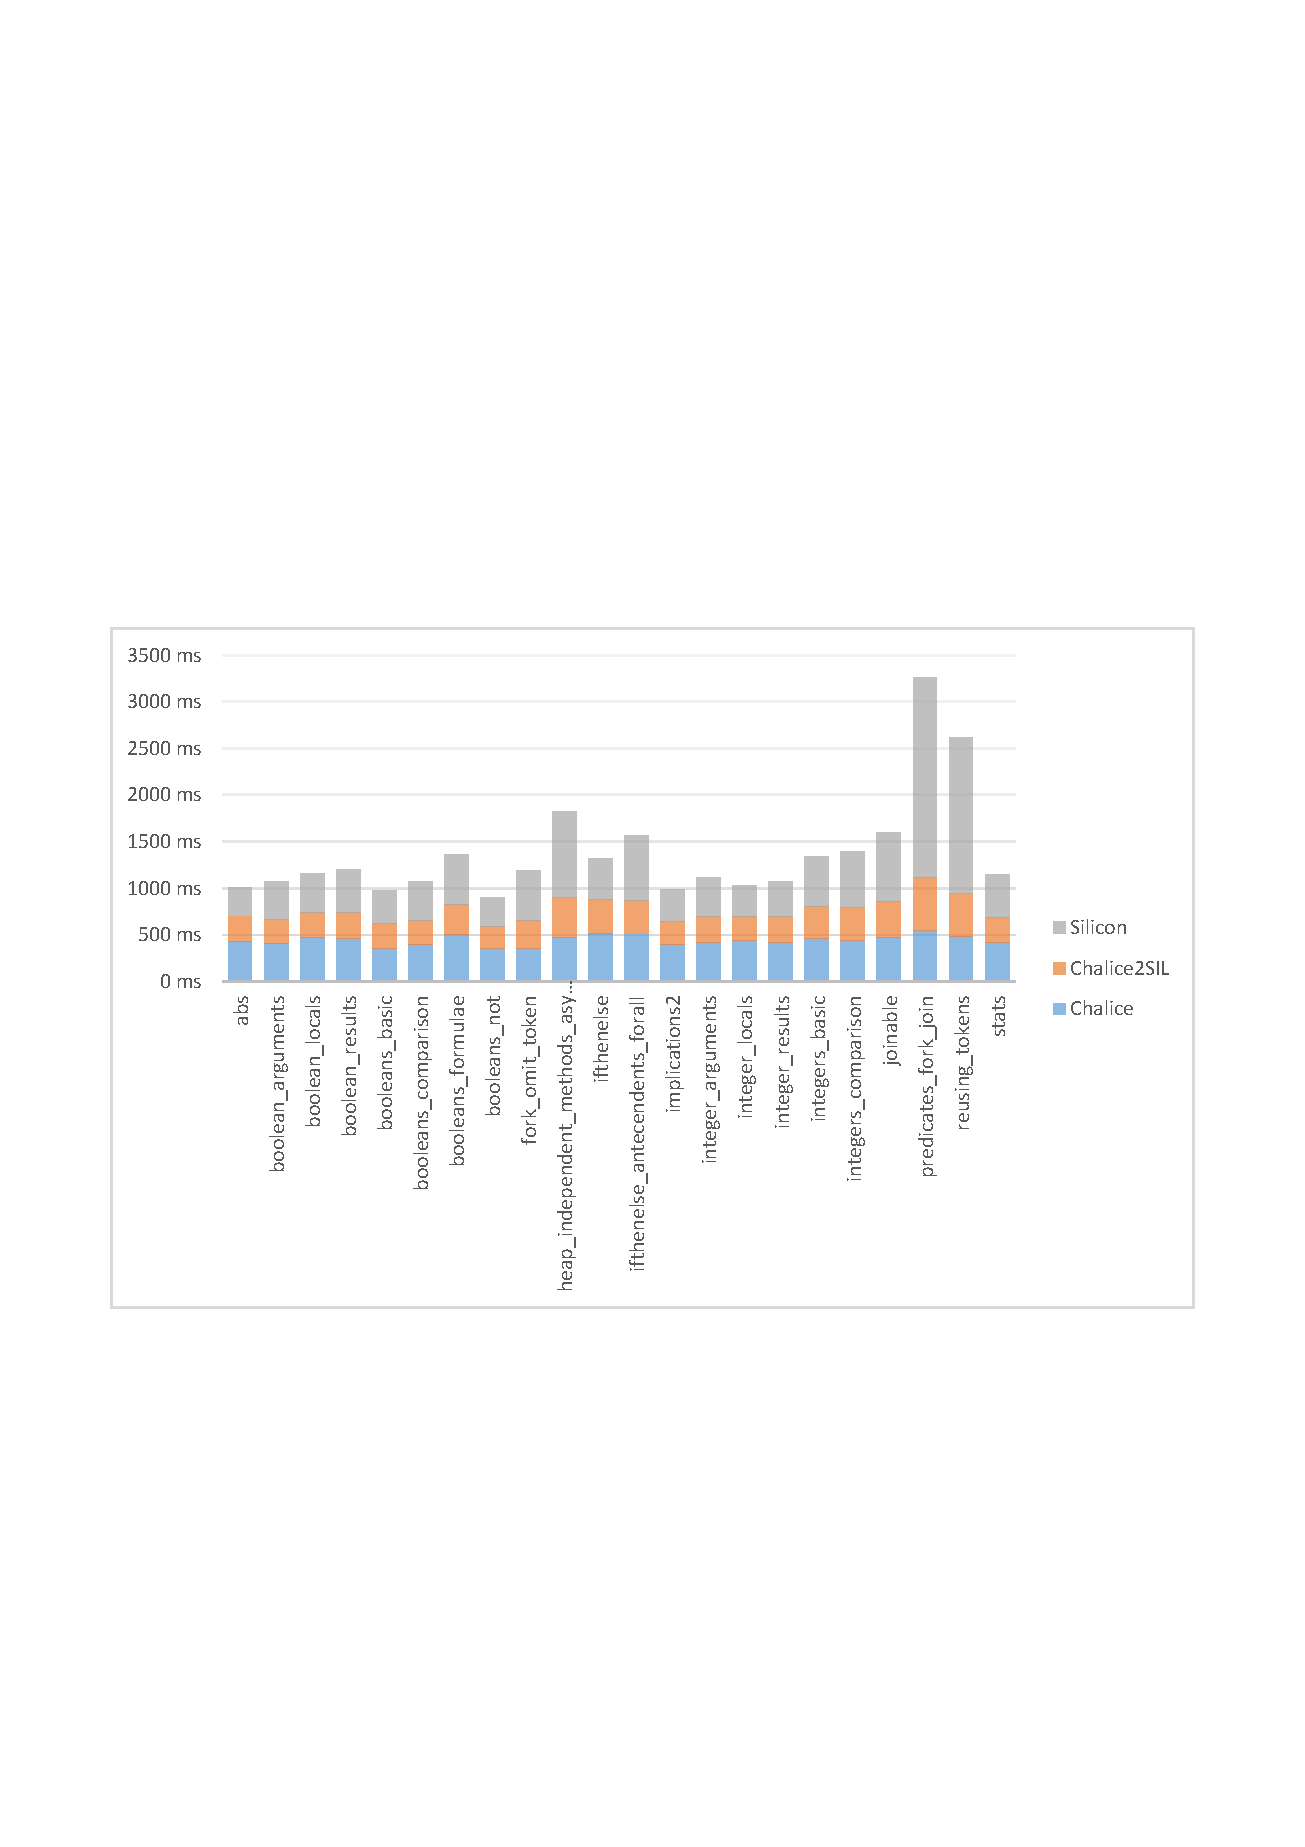
\includegraphics[width=145mm]{src/data/groups-1-3.pdf}
\caption{Running Chalice2SIL+Silicon for tests in \texttt{Basics/}, \texttt{Branching/} and \texttt{ForkJoin/}}\label{fig:perf-grp-1-3}
\end{figure}

\begin{figure}
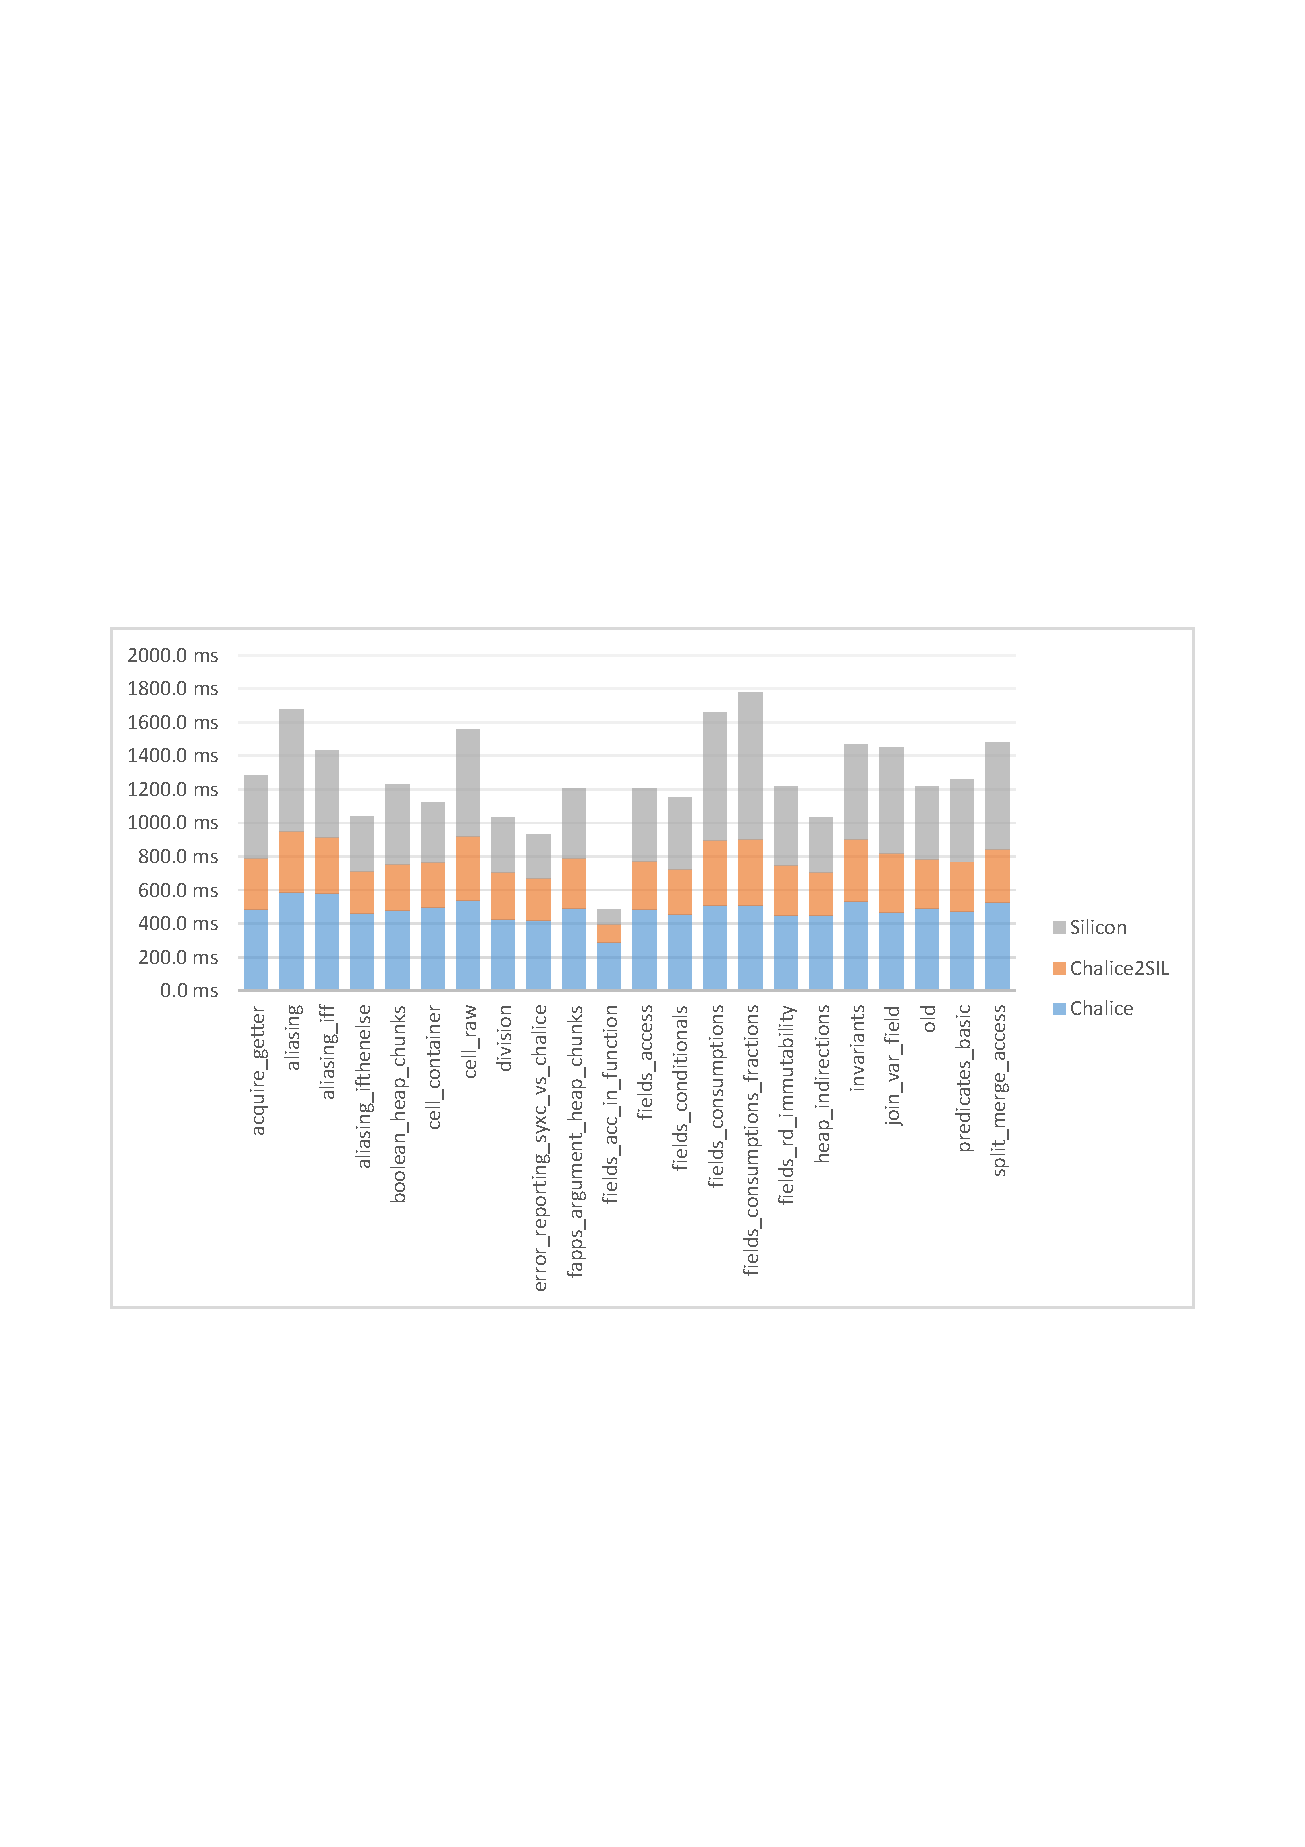
\includegraphics[width=145mm]{src/data/groups-4-6.pdf}
\caption{Running Chalice2SIL+Silicon for tests in \texttt{Heaps/}, \texttt{Misc/} and \texttt{Monitors/}}\label{fig:perf-grp-4-6}
\end{figure}

\begin{figure}
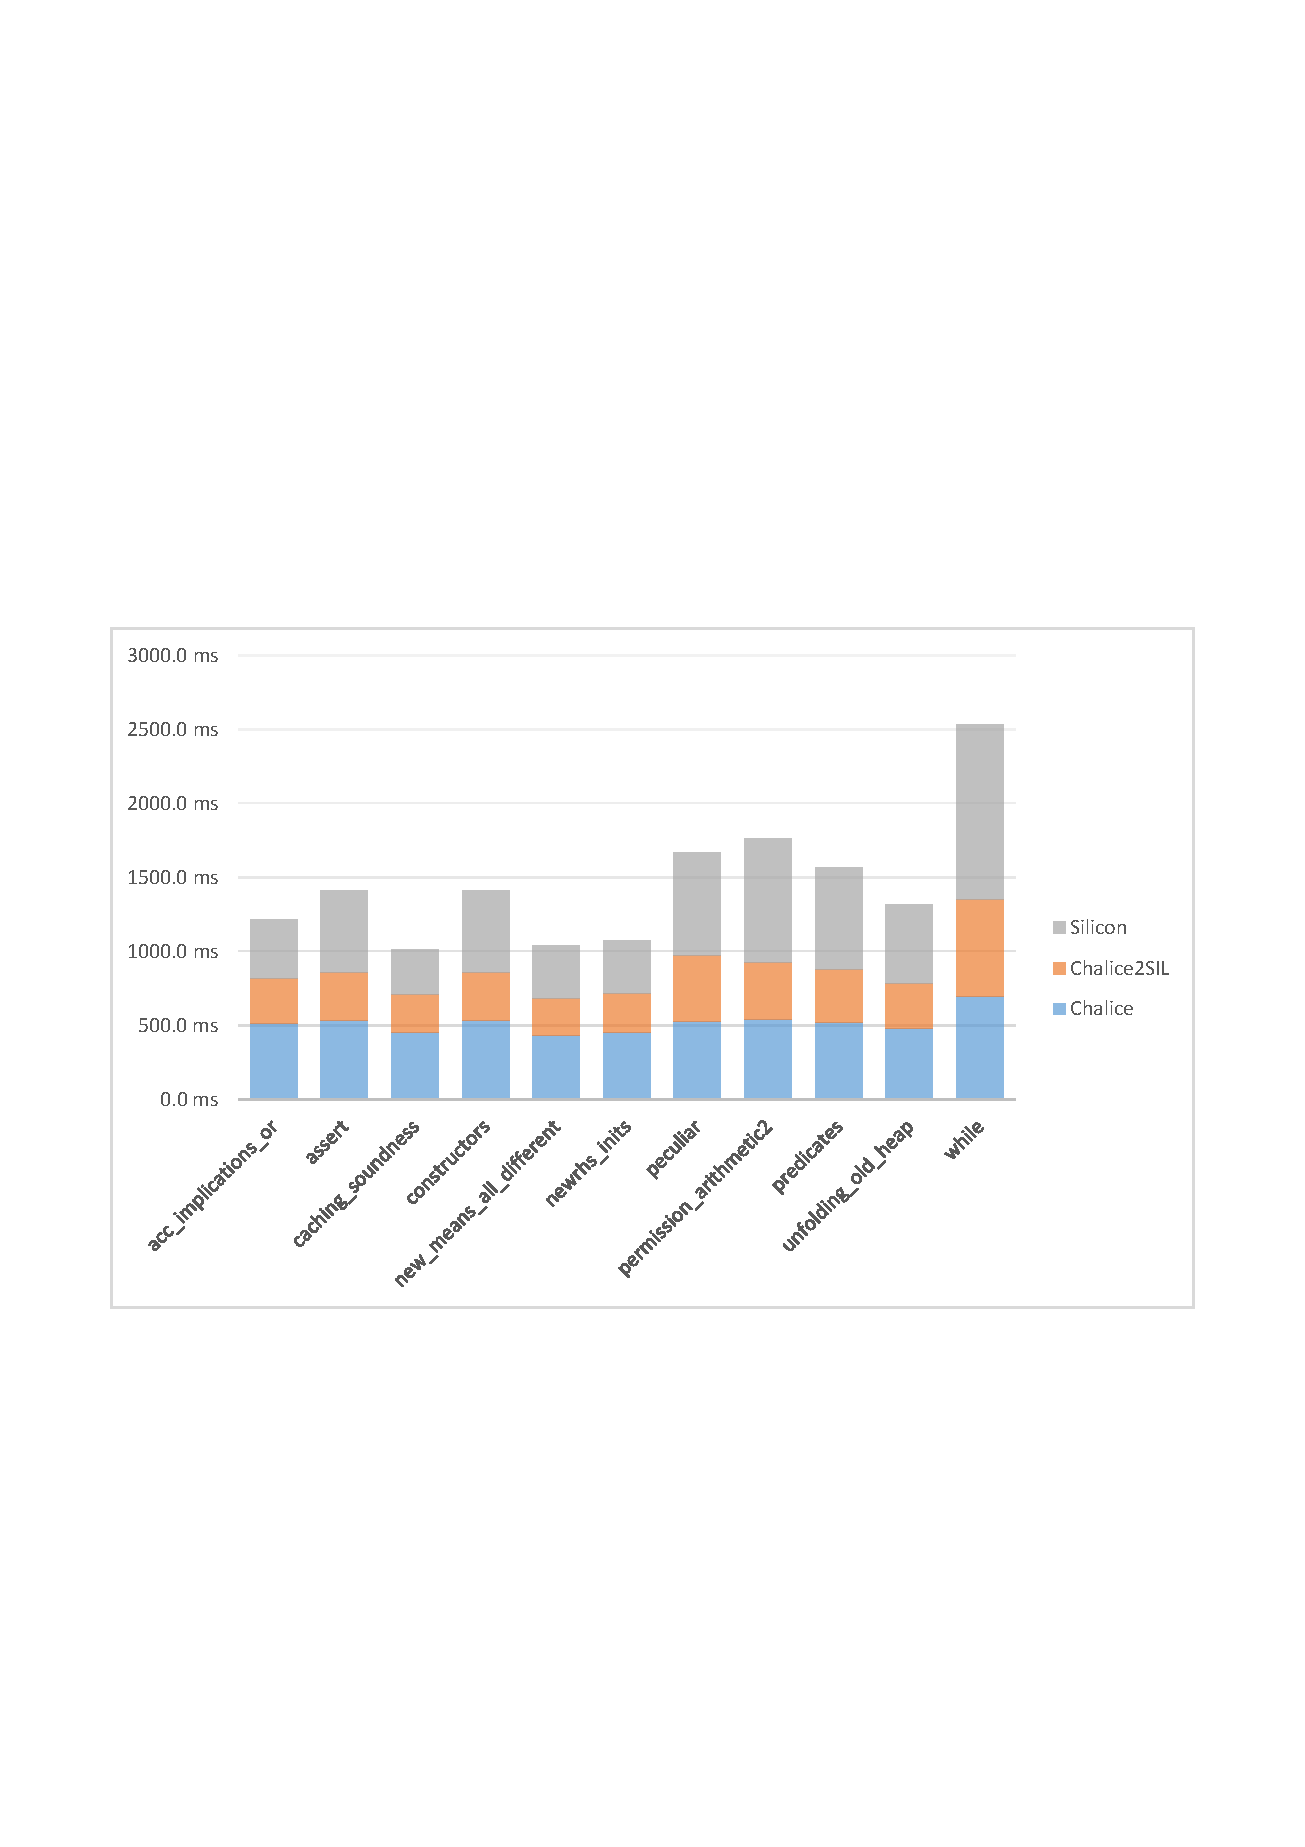
\includegraphics[width=145mm]{src/data/groups-7-8.pdf}
\caption{Running Chalice2SIL+Silicon for tests in \texttt{PermissionModel/}, \texttt{VariousFeatures/}}\label{fig:perf-grp-7-8}
\end{figure}

Figures \ref{fig:perf-grp-1-3}, \ref{fig:perf-grp-4-6} and \ref{fig:perf-grp-7-8} break down the time taken by the Chalice parser/typechecker, Silicon and Chalice2SIL for each test case. 
Constructing the Chalice AST took longer than the translation to SIL in all but two cases: \texttt{ForkJoin/predicates_fork_join} and  \texttt{PermissionModel/basic}.
We omitted the latter from the diagrams for better readability as it is a bit of an outlier with a Silicon runtime of over $4.5\text{s}$ (Syxc only needed $1.2\text{s}$).
It is not clear why verification of this test case via Chalice2SIL+Silicon is that slow. 

As the runtimes of the tests in the benchmark sometimes vary greatly between different test cases, looking at absolute times is not a meaningful way to compare Chalice2SIL and Syxc. 
Instead we look at the factor by which Chalice2SIL+Silicon is slower than Syxc. 
In the majority of cases this factor is between $1.6$ and $1.8$, but there are also cases where Chalice2SIL is $2.5+$ times slower.
Figure \ref{fig:full-ratio-distribution} shows how factors were distributed in this benchmark. 
Two outliers with ratios $3.69$ and $5.02$ were omitted from this diagram in the interest of readability.

\begin{figure}
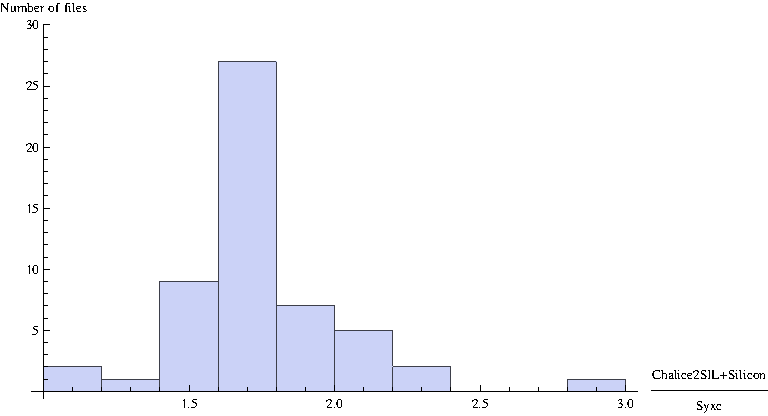
\includegraphics[width=145mm]{src/data/full-ratio-distribution.pdf}
\caption{Distribution of the factor by which Chalice2SIL+Silicon is slower than Syxc}\label{fig:full-ratio-distribution}
\end{figure}

\subsection{Implementation status}
Chalice2SIL implements most of Chalice's core functionality and uses nearly all of the features that SIL has to offer.
However, in addition to monitors and deadlock avoidance there are a number of gaps that still need to be filled to make Chalice2SIL+Silicon a true alternative to Syxc or the original Boogie-based Chalice verifier.

In addition to the tests run as part of the evaluation, we also wrote a set of 94 test programs along with expected results that served as part of an automated test suite during development.
Overall, Chalice2SIL should be considered a prototype with room for improvement, especially in terms of performance. 
